\documentclass[../main.tex]{subfiles}

\begin{document}

\chapter{Die entwickelte Applikation} \label{studnetzApplikation}
Die im Rahmen dieser Arbeit entwickelte Applikation ist für Mobiltelefone mit einer Version des Betriebssystems Android mit einem API Level von 17 und höher entwickelt worden \cite{android:APILevel}. Sie kann darauf installiert und anschliessend ausgeführt werden. Für die Verwendung der Applikation ist eine Verbindung zum Internet notwendig.

\section{Features}
Damit die Applikation auch ihren Zweck erfüllen kann, besitzt sie eine Reihe von Features von welchen Benutzer/Benutzerinnen Gebrauch machen können.

\sloppy
\begin{itemize}
	\item Das \emph{Account-Feature}: Die Applikation bietet den Benutzern/ Benutzerinnen die Möglichkeit, sich einen persönlichen Account zu erstellen und ihn zu personalisieren. Es ist ihnen möglich, auf ihrem Profil ihren Namen, ihre besuchte Schule und ihr Geburtsjahr anzugeben. Weiter können sie auch eine kurze Beschreibung von sich verfassen und sie haben die Möglichkeit, falls sie selber Nachhilfe anbieten wollen, Fächer auszuwählen, in welchen sie das tun möchten. Das Profil ist für andere Benutzer/Benutzerinnen einsehbar. Die meisten Accountdetails können innerhalb der Applikation auch noch nach der Registrierung bearbeitet werden.
	\item Das \emph{Such-Feature}: Es ist registrierten Benutzern/Benutzerinnen möglich, über eine Suchfunktion nach anderen registrierten Benutzern/Benutzerinnen zu suchen. Dabei kann nach dem Namen und nach ausgewählten Fächern gesucht werden. Die gefundenen Profile der verschiedenen Benutzern/ Benutzerinnen können anschliessend angesehen werden.
	\item Das \emph{Chat-Feature}: Sollte der Benutzer/die Benutzerin einen anderen Benutzer oder Benutzerin gefunden haben, mit welchem/welcher er/sie Kontakt aufnehmen möchte, kann ein neuer Chat via das gefundene Profil geöffnet werden. Darin können Benutzer/ Benutzerinnen in Echtzeit kurze Textnachrichten miteinander austauschen. Sollte ein Chat geöffnet sein, kann sowohl der Sender/die Senderin wie auch der Empfänger/die Empfängerin ganz einfach von ihrem eigenen Profil auf ihn zugreifen.
\end{itemize}
\fussy

\section{Benutzeroberfläche und Benutzung}%TODO SCREENSHOT VON MAINPAGE, CHAT, SUCHE, PROFIL, LOGIN UND REGISTER
In diesem Abschnitt soll nun etwas genauer auf die fertige Applikation aus der Sicht eines Benutzers/einer Benutzerin eingegangen werden. Dazu gehört zum einen die Benutzeroberfläche der einzelnen Features wie auch deren Benutzung. Eine Übersicht über die gesamte Applikation findet sich in Abbildung \ref{overview}.
\begin{figure} 
	\centering
	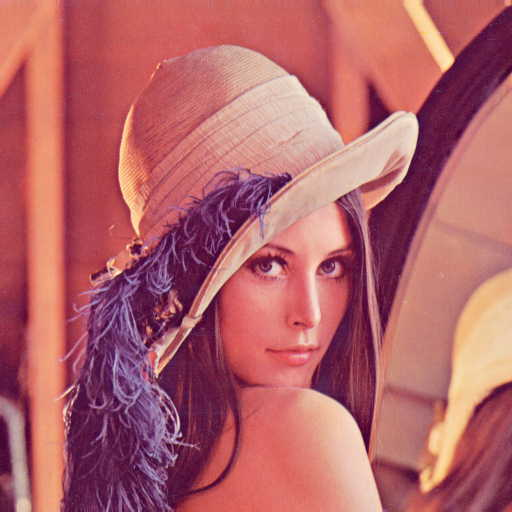
\includegraphics[width=\textwidth, height=0.95\textheight]{./images/lena.jpg}
	\caption{Übersicht aller Screens der Studnetz-Applikation}
	\label{overview}
\end{figure}
%Wenn die Applikation auf dem Mobilgerät ausgeführt wird, öffnet sich der Login-Screen (siehe Abbildung \ref{}). Der Benutzer/Die Benutzerin kann sich nun hier, sollte er/sie bereits einen Account besitzen, mit seinem/ihrem Benutzernamen und Passwort einloggen. Sollte die Person noch keinen Account besitzen, kann sie über einen Schriftzug unterhalb der Logindaten zu einem Registrierungsformular gelangen (siehe Abbildung \ref{}). Im Registrierungsformular wird nach sämtlichen Daten gefragt, die benötigt werden, um einen Account zu erstellen. Dazu gehört ein Benutzername, Vor- und Nachname, eine E-Mail Adresse, ein Passwort, ein Geburtsdatum sowie die momentan besuchte Schule. Ist die Registrierung erfolgreich, kann der Benutzer/die Benutzerin ab sofort sich in seinen/ihren neuen Account einloggen. Nach dem erfolgreichem Einloggen öffnet sich die Hauptseite der Applikation. Sie besteht hauptsächlich aus dem Profil des Benutzers/der Benutzerin (siehe Abbildung \ref{}). Standardmässig findet sich hier ein Profilbild, der Name des Benutzers/der Benutzerin, sein/ihr Geburtsjahr und die besuchte Schule. Diese und noch weitere Angaben wie angebotene Fächer, eine Beschreibung oder ein persönliches Profilbild können in den Einstellungen jederzeit konfiguriert werden, welche über eine Schaltfläche in der oberen rechten Ecke erreicht werden können. Das Profilbild kann dabei entweder direkt mit der Kamera aufgenommen oder aus der Galerie ausgewählt werden. Anschliessend kann der Benutzer/die Benutzerin einen gewünschten ausschnitt im Bild definieren, auf welchen das Bild dann zugeschnitten wird (siehe Abbildung \ref{} und \ref{}). Die ausgewählten Fächer werden in Form von Emblems auf dem Profil dargestellt. Ebenfalls auf der Hauptseite findet sich ein ausfahrbares \emph{BottomSheet} am unteren Ende des Bildschirms. Es kann über eine runde Schaltfläche in der Mitte oder ein einfaches Streichen nach oben ausgefahren werden. Im BottomSheet selber finden sich Einträge für alle offenen Chats des Benutzers/der Benutzerin(siehe Abbildung \ref{}). Über einen einfachen Klick können sie geöffnet werden (siehe Abbildung \ref{}). Das BottomSheet ist auch der Ort, an welchem ein Benutzer/eine Benutzerin sehen kann, ob er/sie neue Nachrichten empfangen hat. Neben dem BottomSheet findet sich ebenfalls im rechten unteren Ende eine runde Schaltfläche mit einer Lupe. Über sie kann auf das Such-Feature zugegriffen werden, welche den Benutzer/die Benutzerin auf einen neuen Screen führt. Dort können die Kriterien für die Suche definiert werden (siehe Abbildung \ref{}). Hier können Suchparameter wie Name und Fächer angegeben werden, nach welchen gesucht werden soll. Ist der Benutzer/die Benutzerin zufrieden mit den Einstellungen kann über eine Schaltfläche die Suche ausgeführt werden. Alle Suchergebnisse werden in Form einer Liste daraufhin im Client aufgeführt (siehe Abbildung \ref{}). Sollte den Benutzer/die Benutzerin Interesse an einem der Ergebnisse haben, kann durch einfaches Auswählen des Elementes in der Liste das Profil des/der gefundenen Benutzer/Benutzerin aufgerufen werden (siehe Abbildung \ref{}). Ist der Benutzer/die Benutzerin interessiert, Kontakt mit dem/der gefundenen Benutzer/Benutzerin aufzunehmen, kann nun über eine Schaltfläche auf dem Profil ein neuer Chat geöffnet werden (siehe Abbildung \ref{}). Dort können dann mithilfe kurzer Textnachrichten genauere Informationen über eine mögliche Zusammenarbeit ausgetauscht werden. Die Überlieferung erfolgt dabei in Echtzeit.


\subsubsection*{Login und Registrierung}
Beim Ausführen der Applikation auf dem Mobilgerät wird der Benutzer/die Benutzerin vom Login-Screen der Applikation begrüsst (siehe Abbildung \ref{login_register}). Der Benutzer/die Benutzerin kann sich nun hier, sollte er/sie bereits einen Account besitzen, mit seinem/ihrem Benutzernamen und Passwort einloggen. Sollte die Person noch keinen Account besitzen, kann sie über einen Schriftzug unterhalb der Logindaten zu einem Registrierungsformular gelangen (siehe Abbildung \ref{login_register}). Im Registrierungsformular wird nach sämtlichen Daten gefragt, die benötigt werden, um einen Account zu erstellen. Dazu gehört ein Benutzername, Vor- und Nachname, eine E-Mail Adresse, ein Passwort, die momentan besuchte Schule sowie die aktuelle Klassenstufe der besuchten Schule. Mit Klassenstufe ist dabei die Klassenstufe gemeint, auf welcher man sich an der momentanen Schule befindet. Wenn ein Benutzer/eine Benutzerin beispielsweise das 3. Jahr an der KSA besuchen würde, befände sie sich in der 3. Klasse. Für Schülerinnen und Schüler der gleichen Schule sollte somit einfacher zu erkennen sein, auf welcher Stufe sich ein anderer registrierter Schüler/eine andere registrierte Schülerin befindet. Da nicht alle Schulen die gleiche Anzahl an Stufen besitzen, passen sich die auswählbaren Stufen innerhalb der Applikation jeweils an die ausgewählte Schule an. So besitzt die KSA beispielsweise vier Stufen, während das Gymnasium Einsiedeln sechs besitzt. Ist die Registrierung erfolgreich, kann sich der Benutzer/die Benutzerin ab sofort in seinen/ihren neuen Account einloggen.

\begin{figure} 
	\centering
	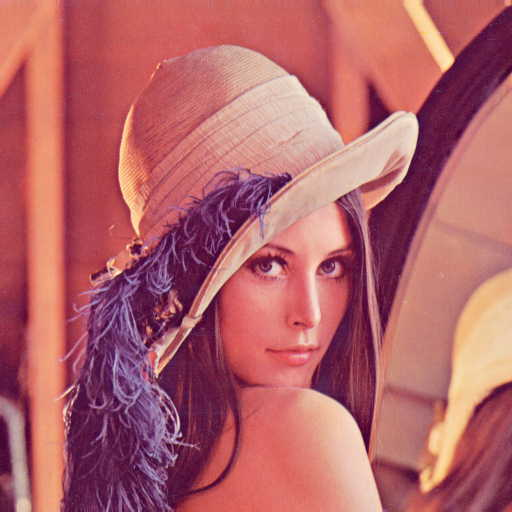
\includegraphics[width=0.45\textwidth*2, height=0.45\textwidth/9*16]{./images/lena.jpg}
	\caption{Links: Loginformular, Rechts: Registrierungsformular}
	\label{login_register}
\end{figure}

\subsubsection*{Navigation}
Die Navigation innerhalb der Applikation nach einem erfolgreichen Login erfolgt hauptsächlich über eine sogenannte \emph{Bottom Navigation}. Dort können jederzeit bei der Benutzung der Applikation zwischen den wichtigsten Screen hin und her gewechselt werden. Die Studnetz-Applikation besitzt drei solche Screens, welche in den folgenden Paragraphen genauer erläutert werden. Weiter ist es meist möglich, über eine Schaltfläche in der oberen, linken Ecke einen Schritt zurück zu gehen, sollte dies von Bedarf sein.

\subsubsection*{Benutzerprofil, Einstellungen und Hauptseite} 
Dieser Screen ist der, welcher nach einem erfolgreichen Login angezeigt wird. Er besteht aus dem Profil des Benutzers/der Benutzerin (siehe Abbildung \ref{mainpage}). 
\begin{figure} 
	\centering
	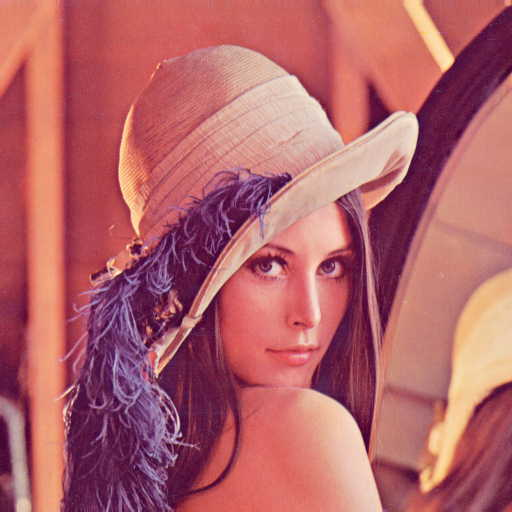
\includegraphics[width=0.45\textwidth, height=0.45\textwidth/9*16]{./images/lena.jpg}
	\caption{Hauptseite mit Profil des Benutzers/der Benutzerin}
	\label{mainpage}
\end{figure}
Standardmässig findet sich hier ein standardmässiges Profilbild, der volle Name des Benutzers/der Benutzerin, die besuchte Schule sowie die Klassenstufe. Diese und noch weitere Angaben wie angebotene Fächer, eine Beschreibung oder ein persönliches Profilbild können in den Einstellungen, welche über eine Schaltfläche in der oberen rechten Ecke in der Toolbar erreicht werden können, jederzeit konfiguriert werden. Das Profilbild kann dabei entweder direkt mit der Kamera aufgenommen oder aus der Galerie des Mobiltelefons ausgewählt werden. Anschliessend kann der Benutzer/die Benutzerin einen gewünschten Ausschnitt im Bild definieren, auf welchen das Bild dann zugeschnitten wird (siehe Abbildung \ref{choose_crop}). Die ausgewählten Fächer werden in Form von Emblems auf dem Profil dargestellt.
\begin{figure} 
	\centering
	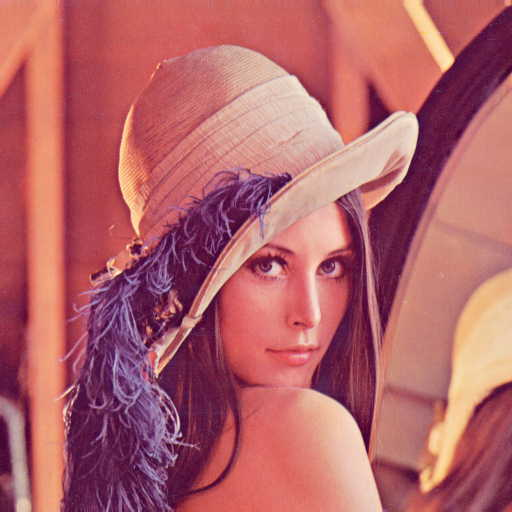
\includegraphics[width=0.45\textwidth*2, height=0.45\textwidth/9*16]{./images/lena.jpg}
	\caption{Links: Auswahl einer Quelle für das Bild, Rechts: Zuschneiden des Bildes}
	\label{choose_crop}
\end{figure}

\subsubsection*{Suche}
Das Suchfeature der Applikation findet sich in Form eines in vier Stufen unterteilten Prozess. Das Suchfeature kann über die Bottom Navigation erreicht werden. Sollte ein Benutzer/eine Benutzerin mitten in der Suche das Suchfenster verlassen habe, wird der momentane Stand gespeichert und wenn die Suche wieder aufgerufen wird, kann an der Stelle weitergemacht werden, wo zuletzt aufgehört wurde. Die erste Stufe der Suche findet sich dabei in Form eines Screens, wo Suchkriterien wie Name, Schule, Stufe und angebotene Fächer definiert werden können, nach welchen gesucht werden soll (siehe Abbildung \ref{searchOverview}).
\begin{figure} 
	\centering
	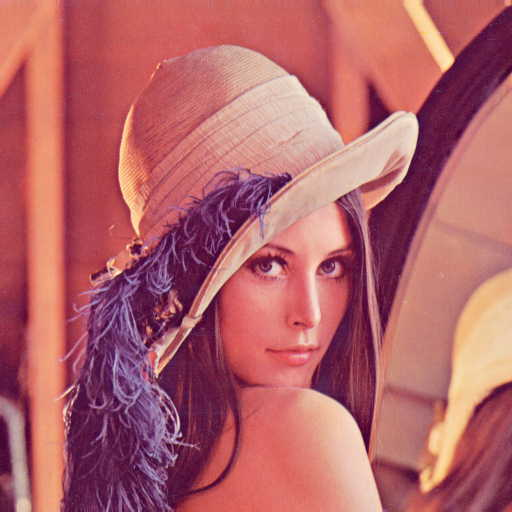
\includegraphics[width=0.45\textwidth, height=0.45\textwidth/9*16]{./images/lena.jpg}
	\caption{Filtereinstellungen für die Suche}
	\label{searchOverview}
\end{figure} 
Ist der Benutzer/die Benutzerin zufrieden mit den Konfigurationen der Suche, kann über eine Schaltfläche die Suche ausgeführt werden und der Screen ändert sich zur zweiten Stufe, wo die Suchergebnisse in Form einer Liste dargestellt werden (siehe Abbildung \ref{results_profile}). Erweckt ein Ergebnis der Suche das Interesse des Benutzers/der Benutzerin, kann über das Auswählen eines Ergebnises das Profil des gefundenen Benutzers/der gefundenen Benutzerin geöffnet werden, womit man sich dann auf der dritten Stufe befindet (siehe Abbildung  \ref{results_profile}). Von dort kann dann ein neuer Chat über eine Schaltfläche eröffnet werden, wo dann genauere Informationen über die mögliche Zusammenarbeit ausgetauscht werden können. Der Chat bildet dann somit die vierte Stufe der Suche.

\begin{figure} 
	\centering
	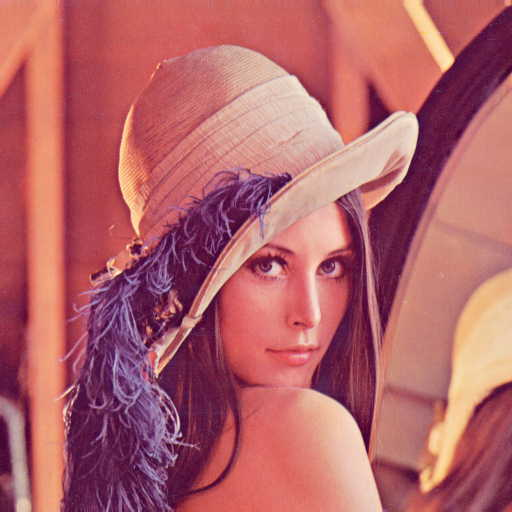
\includegraphics[width=0.45\textwidth*2, height=0.45\textwidth/9*16]{./images/lena.jpg}
	\caption{Links: Auflistung der Suchergebnisse, Rechts: Profil eines Benutzers}
	\label{results_profile}
\end{figure}

\subsubsection*{Chats}
Ebenfalls über die Bottom Navigation kann ein Screen geöffnet werden, wo alle Chats angezeigt werden, in welchen ein Benutzer/eine Benutzerin involviert ist. Die angezeigten Chats in der Übersicht zeigen jeweils die Profilbilder der Chatpartner/ Chatpartnerinnnen und die zuletzt gesendete Nachricht an (siehe Abbildung \ref{chat}). Durch das Auswählen eines Elements der Übersicht kann ein gewünschter Chat geöffnet werden (siehe Abbildung \ref{chat}). Die Überlieferungen der Nachrichten im Chat erfolgen in Echtzeit, was eine flüssige Kommunikation zwischen zwei Benutzern/Benutzerinnen ermöglicht.

\begin{figure} 
	\centering
	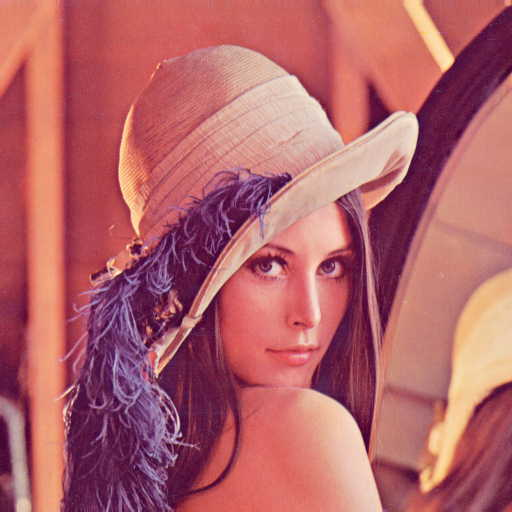
\includegraphics[width=0.45\textwidth*2, height=0.45\textwidth/9*16]{./images/lena.jpg}
	\caption{Links: Auflistung der offenen Chats, Rechts: Offener Chat}
	\label{chat}
\end{figure}

\end{document}